\documentclass[12pt]{article}

\usepackage{bbm}
\usepackage{fancyhdr}
\usepackage{titling}
\usepackage{enumitem}
\usepackage{amsmath}
\usepackage{dsfont}
\usepackage{amsfonts}
\usepackage{amssymb}
\usepackage{amsthm}
\usepackage{geometry}
\usepackage{tikz}
\usepackage{algorithm}
\usepackage{algpseudocode}
\geometry{verbose,tmargin=1in,bmargin=1in,lmargin=1in,rmargin=1in}
\renewcommand{\vec}[1]{\mathbf{#1}}
\newcommand{\dec}{\text{dec}}
\newcommand{\divi}{\mathbin{\textnormal{div}}}
\title{Homework 1}
\author{Satvik Prasad}
\date{}
\newtheorem{lemma}{Lemma}[section]
\fancypagestyle{plain}{%
  \fancyhf{}
  \fancyhead[L]{\theauthor}
  \fancyhead[R]{\thedate}
}
\pagestyle{plain}
\makeatletter
\def\@maketitle{%
  \newpage
  \null
  \vskip 1em%
  \begin{center}%
    \let \footnote \thanks
    {\LARGE \@title \par}%
    \vskip 1em%
  \end{center}%
  \par
\vskip 1em}
\makeatother
\usepackage{cmbright}

\newcommand{\mat}[1]{\mathbf{#1}}

% ---------- Probability theory ----------
% Core operators (optional argument-free; use as \E{X}, \Var{X}, \Cov{X}{Y})
\DeclareMathOperator{\EOp}{\mathbb{E}}
\DeclareMathOperator{\VarOp}{Var}
\DeclareMathOperator{\CovOp}{Cov}
\DeclareMathOperator{\CorrOp}{Corr}

\renewcommand{\P}[1]{\mathbb{P}\left(#1\right)}        % \P{A}
\newcommand{\E}[1]{\EOp\left[#1\right]}                % \E{X}
\newcommand{\Var}[1]{\VarOp\left(#1\right)}            % \Var{X}
\newcommand{\Cov}[2]{\CovOp\left(#1,\,#2\right)}       % \Cov{X}{Y}
\newcommand{\Corr}[2]{\CorrOp\left(#1,\,#2\right)}     % \Corr{X}{Y}
\newcommand{\SD}[1]{\operatorname{SD}\left(#1\right)}  % \SD{X}

% Subscripted versions, e.g. \Esub{\theta}{X}, \Psub{\theta}{A}
\newcommand{\Esub}[2]{\EOp_{#1}\left[#2\right]}
\newcommand{\Psub}[2]{\mathbb{P}_{#1}\left(#2\right)}

% Conditioning, indicators, independence
\newcommand{\given}{\,\middle|\,}                      % \E{X \given Y}
\newcommand{\ind}[1]{\mathbbm{1}\left\{#1\right\}}     % \ind{X > 0}
\newcommand{\indep}{\perp\!\!\!\perp}                  % X \indep Y
\newcommand{\iid}{\overset{\text{iid}}{\sim}}          % X_i \iid \Normal(0,1)

% Convergence
\newcommand{\convp}{\xrightarrow{\;p\;}}               % in probability
\newcommand{\convd}{\xrightarrow{\;d\;}}               % in distribution
\newcommand{\convas}{\xrightarrow{\text{a.s.}}}        % almost surely
\newcommand{\convLp}[1]{\xrightarrow{L^{#1}}}          % in L^p

% Probability spaces
\newcommand{\F}{\mathcal{F}}                           % sigma-algebra
\newcommand{\B}{\mathcal{B}}                           % Borel sigma-algebra
\newcommand{\pspace}{(\Omega, \F, \mathbb{P})}

% Common distributions
\newcommand{\Normal}{\mathcal{N}}
\newcommand{\Bern}{\operatorname{Bernoulli}}
\newcommand{\Bin}{\operatorname{Binomial}}
\newcommand{\Pois}{\operatorname{Poisson}}
\newcommand{\Unif}{\operatorname{Uniform}}
\newcommand{\Exp}{\operatorname{Exp}}
\newcommand{\Geom}{\operatorname{Geometric}}
\newcommand{\Gam}{\operatorname{Gamma}}
\newcommand{\Beta}{\operatorname{Beta}}

% Number sets
\newcommand{\R}{\mathbb{R}}
\newcommand{\N}{\mathbb{N}}
\newcommand{\Z}{\mathbb{Z}}


\begin{document}
\begin{enumerate}
    \item Let $x_2 = \mu \in \mathbb R$ and $x_4 = \lambda \in \mathbb R,$ meaning for all $u \in U,$ there exist $\mu, \lambda \in \mathbb R$ such that
    $$
    u = (3\mu, \mu, 7\lambda, \lambda).
    $$
    Since $U$ is a vector space, we get 
    $$
    u = \mu \begin{pmatrix}
    3 \\
    1 \\
    0 \\
    0
    \end{pmatrix} + \lambda \begin{pmatrix}
        0 \\
        0 \\
        7 \\ 
        1
    \end{pmatrix}.
    $$
    Since $\langle 3, 1, 0, 0 \rangle$ and $\langle 0, 0, 7, 1\rangle$ are linearly independent, and for all $u$ there exist coefficients such that $u$ is a linear combination of these vectors, the set
    $$
    \{\langle 3, 1, 0, 0 \rangle, \langle 0, 0, 7, 1\rangle\}
    $$
    is a basis for $U.$

    \item Assume we have some $U \subseteq \mathbb R^3$ as a subspace. Then, since $\dim U \leq \dim \mathbb R^3,$ we have 4 cases:
    \begin{itemize}
        \item If $\dim U = 0,$ then the only possibility for $U$ is $\{0\},$
        
        \item If $\dim U = 1,$ then every basis can be written in the form $\{\vec b\}$ for some vector $\vec b \neq 0,$ meaning every element in $U$ can be written as $\lambda \vec b$ for some $\lambda \in \mathbb R.$ Hence, $U$ is the line through the origin in the direction of $\vec b.$

        \item If $\dim U = 2,$ then there is some basis $\{\vec b_1, \vec b_2\}$ such that there are $\lambda, \mu \in \mathbb R,$ for all $u \in U$ such that $u = \lambda \vec b_1 + \mu \vec b_2.$ Hence, this is a plane through the origin with normal vector $\vec b_1 \times \vec b_2$ (non-zero since $\vec b_1, \vec b_2$ linearly independent).

        \item If $\dim = 3,$ then there is a basis $\{\vec b_1, \vec b_2, \vec b_3\}$ such that for all $u \in U,$ there are $\mu, \lambda, \nu$ such that $$
        u = \lambda \vec b_1 + \mu \vec b_2 + \nu \vec b_3.
        $$
        Since $\vec b_1, \vec b_2, \vec b_3$ are three linearly independent vectors in $\mathbb R^3,$ the matrix 
        $$
        \begin{pmatrix}
        \vec b_1 & \vec b_2  & \vec b_3
        \end{pmatrix}
        $$
        has rank $3,$ meaning it is invertible, and there exist coefficients $\lambda, \mu, \nu$ for all $v \in \mathbb R^3$ such that $\lambda \vec b_1 + \mu \vec b_2 + \nu \vec b_3 =v .$ In other words, this basis spans $\mathbb R^3,$ and hence $U = \mathbb R^3.$
    \end{itemize}

    \item Let $U = \{\mathcal P_4(\mathbb R) \mid \int_{-1}^{1} p(x) \, dx = 0\}.$ Since $1, x, x^2, x^3, x^4$ are a basis for $\mathcal P_4(\mathbb  R),$ we can conclude for all $p \in \mathcal P_4(\mathbb R),$ 
    $$
    p(x) = a_0 + a_1 x + a_2 x^2 + a_3 x^3 + a_4 x^4
    $$
    for coefficients $a_0, a_1, \ldots, a_4 \in \mathbb R.$ Then, for 
    \begin{align*}
    0 = \int_{-1}^{1} p(x) \, dx &= \int_{-1}^{1} a_0 + a_1 x + a_2 x^2 + a_3 x^3 + a_4 x^4 \, dx \\
    &=  2a_0 + \frac{2}{3}a_2 + \dfrac{2}{5} a_4 x^4.
    \end{align*}
    Thus, we need 
    $$
    a_0 = - \frac{1}{3}a_2 - \frac{1}{5} a_4
    $$
    for all $p \in U.$ Hence, for all $p \in U,$ there exist coefficients $a_1, a_2, a_3, a_4 \in \mathbb R$ such that
    \begin{align*}
        p(x) &= -\frac{1}{3} a_2 - \frac{1}{5} a_4 + a_1 x + a_2 x^2 + a_3 x^3 + a_4 x^4 \\
        &= a_1 x + a_2 \left(x^2 - \frac{1}{3}\right) + 
        a_3 x^3 + 
        a_4\left(x^4 - \frac{1}{5}\right)
    \end{align*}
    This means $x, x^2 - 1/3, x^3, x^4 - 1/5$ span $U.$ Since they are linearly independent, we can conclude
    $$
    \left\{
    x, x^2 - \frac{1}3{}, x^3, x^4 - \frac{1}{5}
    \right\}
    $$
    are a basis for $U.$

    \item For the sake of contradiction, assume that $U + W$ is not a direct sum. Then, there exists a non-zero $u \in U, w \in W$ such that $u + w = 0$ such that $u + w = 0.$ Then, consider the basis sets of $U, W$ respectively:
    $$
    \{u_1, u_2, u_3\}, \{w_1, \ldots, w_5\}.
    $$
    Thus, $u = a_1 u_1 + a_2 u_2 + a_3 u_3$ for coefficients $(a_1, \ldots, a_3) \in \mathbb R^3 \setminus \{0\},$ and 
    $$
    w = b_1 w_1 + \ldots + b_5 w_5.
    $$ for $(b_1, \ldots, b_5) \in \mathbb R^{5} \setminus \{0\}.$ Hence, since $u + w  = 0,$ we have
    $$
    a_1 u_1 + a_2 u_2 + a_3 u_3 + b_1 w_1 + \ldots + b_5 w_5 = 0
    $$
    for some $(a_1, a_2, a_3, b_1, \ldots, b_5) \in \mathbb R^{8} \setminus \{0\},$ meaning $A = \{u_1, u_2, u_3, w_1, \ldots, w_5\}$ are not linearly independent. However, since for any $v \in U + W,$ we can write 
    $$
    v = \lambda_1 u_1 + \lambda_2 u_2 + \lambda_3 u_3 + \lambda_4 w_1 + \ldots + \lambda_8 w_5,
    $$
    and thus $A$ spans $U + W.$ Since $A$ is not linearly independent, remove some $a \in A$ that is a linear combination of the remaining elements, yielding set $A'$ with $|A'| = 7.$ Since the removed vector $a'$ is in the span of the remaining elements, removing it maintains $A'$ spanning $U + W.$ If $A'$ is still linearly dependent, repeat this process until we get a linearly independent basis set $A^\star$ that spans $U + W.$ Since this process occurred at least once, $|A^\star| < 8,$ meaning $8 = \dim \mathbb R^8 = \dim (U + W) < 8,$ which is a contradiction.

    Therefore, $U + W$ must be a direct sum $U \oplus W.$

    \item Assume we have some finite dimensional $V$ with $\dim V = n \geq 1.$ Construct an arbitrary basis for $V,$
    $$
    \{v_1, \ldots, v_n\}.
    $$
    Then, construct subspaces $V_k$ such that
    $$
    V_k = \{\lambda v_k : \lambda \in \mathbb F\}
    $$
    for all $1 \leq k \leq n.$ We prove that $$
    V = V_1 \oplus V_2 \oplus \ldots \oplus  V_n.
    $$

    To do this, consider the sum of some arbitrary 
    $$
    \underbrace{(V_1 \oplus \ldots \oplus V_{j - 1})}_{V_{<j}} + V_{j},
    $$
    for $1 < j \leq n.$ By the definition of a sum, for all $v \in V_{< j},$  we can write $v$ as 
    $$
    \lambda_1 v_1  + \lambda_2 v_2 + \ldots + \lambda_{j -1 } v_{j -1}
    $$
    for coefficients in $\mathbb F.$ Additionally, for $u \in V_j$ we can write 
    $u = \lambda_j v_j.$ Assume this is not a direct sum, i.e there are non-zero $v \in V_{<j}, u \in V_j$ such that
    $u + v = 0.$

    Then, there are coefficients such that
    $$
    \sum_{k = 1}^{j}\lambda_k v_k = 0
    $$
    for $(\lambda_1, \ldots, \lambda_{j-1}) \in \mathbb R^{j-1} \setminus \{0\}$ and $\lambda_j \neq 0.$ However, this contradicts the linear independence of the basis for $V,$ meaning $V_{<j} + V_j$ must be a direct sum for all $2 \leq j \leq n.$ Therefore, all sums are direct sums (reading left to right), meaningn there exist $V_1, \ldots, V_n$ such that
    $$V = V_1 \oplus V_2 \oplus \ldots \oplus V_n.$$
\end{enumerate}

\subsection{Evaluating Proofs}
This proof is incorrect. The correct formula is 
$$
\dim (U + W) = \dim U + \dim W - \dim (U \cap W),
$$
but $U + W$ is not necessarily equal to $V.$

\subsection{Using Computers}
    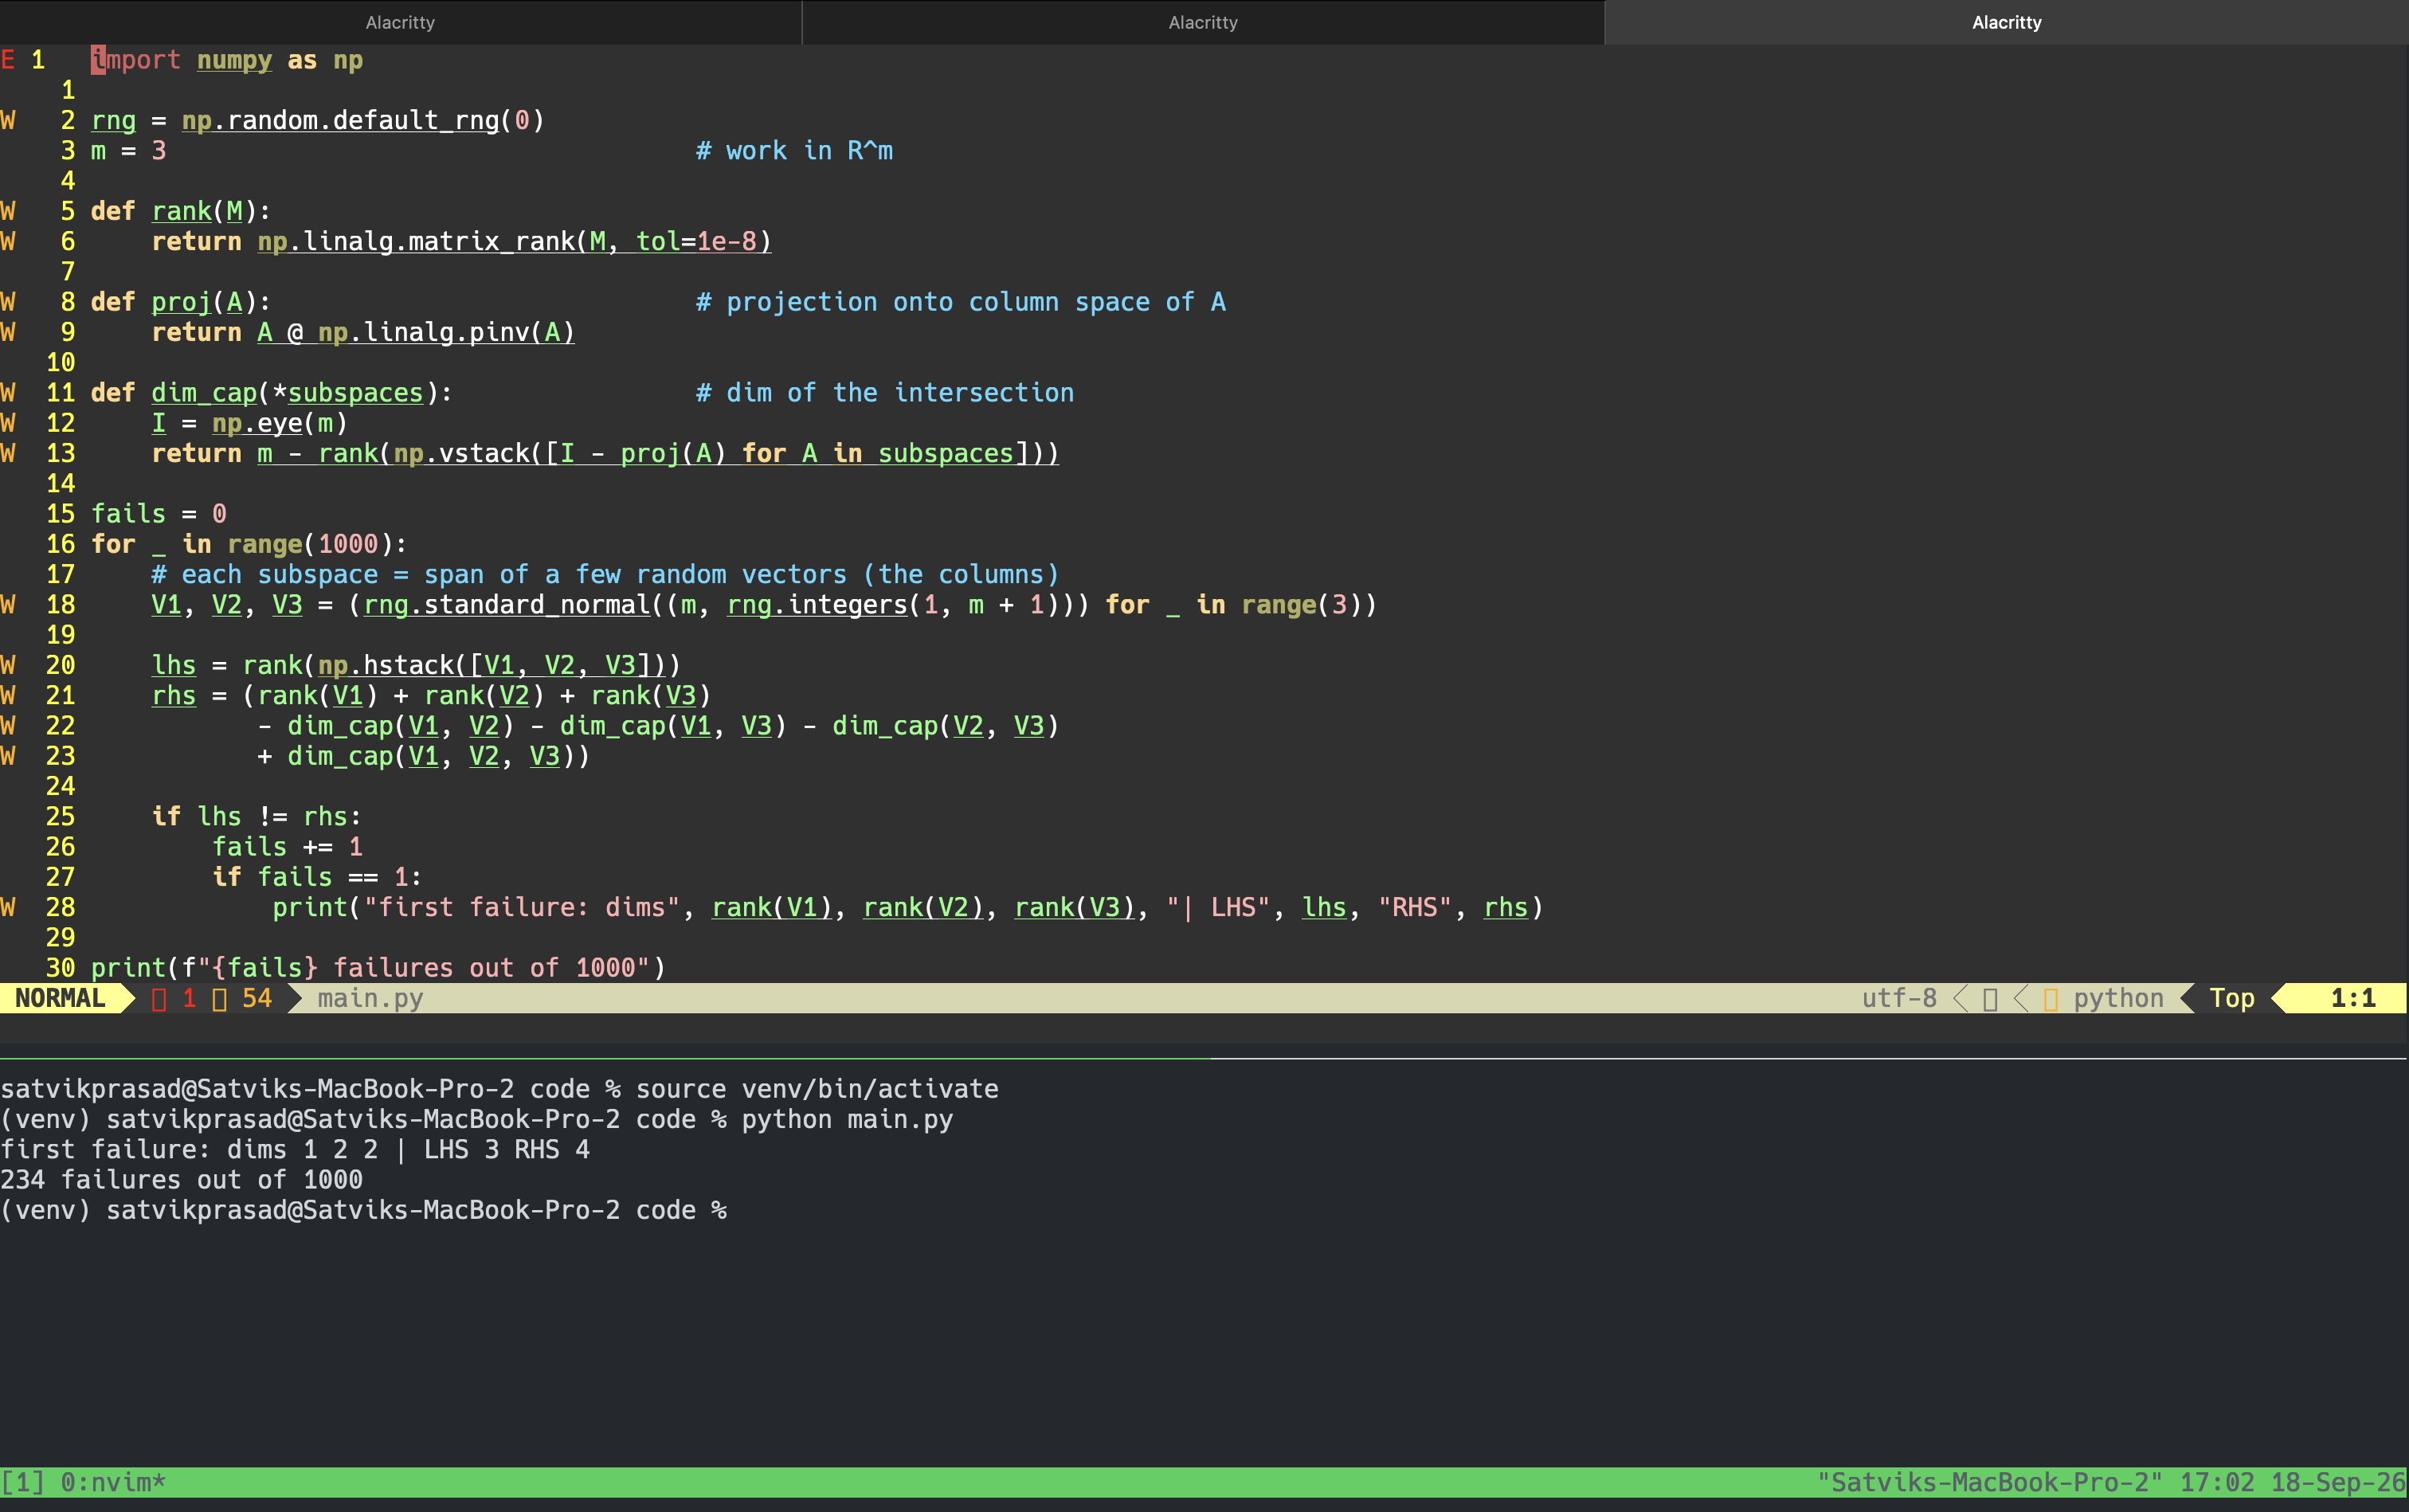
\includegraphics[width=\linewidth]{Screenshot 2026-09-18 at 5.02.51 pm.png}

Claim is false, with counterexample of 3 lines in the same plane who only share the origin.

\end{document}